\newpage
\setlength{\parskip}{1em}
\section{Object tracking: 3D Kalman Filter}
\label{sec:kal}
\subsection{Theoretical concept of the algorithm}
Once the object is detected it is need to know how reliable is the recognition. If there is a fail in the object detection that will may lead to wrong path planning which could make the robot hit the ball. In order to avoid that, a Kalman Filter is implemented for tracking the motion of the ball.\par
The Kalman Filter is a statistical algorithm which uses several measurements observed to produce estimates that in the end will predict the next state of the ball.\par
The algorithm has two step process (see fig.\ref{fig:kf_sch}). First there is a prediction step which will estimate the next state of the ball along with the measurement and process uncertainties. Once the state is predicted a new measurement related to the predicted state is received. When the measurement is observed the state of the ball is corrected by updating the estimates using a weighted average. The purpose of using a weighted average is that the model will rely more on the data points that has less uncertainty. In practical view, a failure in object detection will not affect that much the performance of the detection.
\begin{figure}[ht!]
    \centering
    \captionsetup{justification=centering,margin=1cm}
    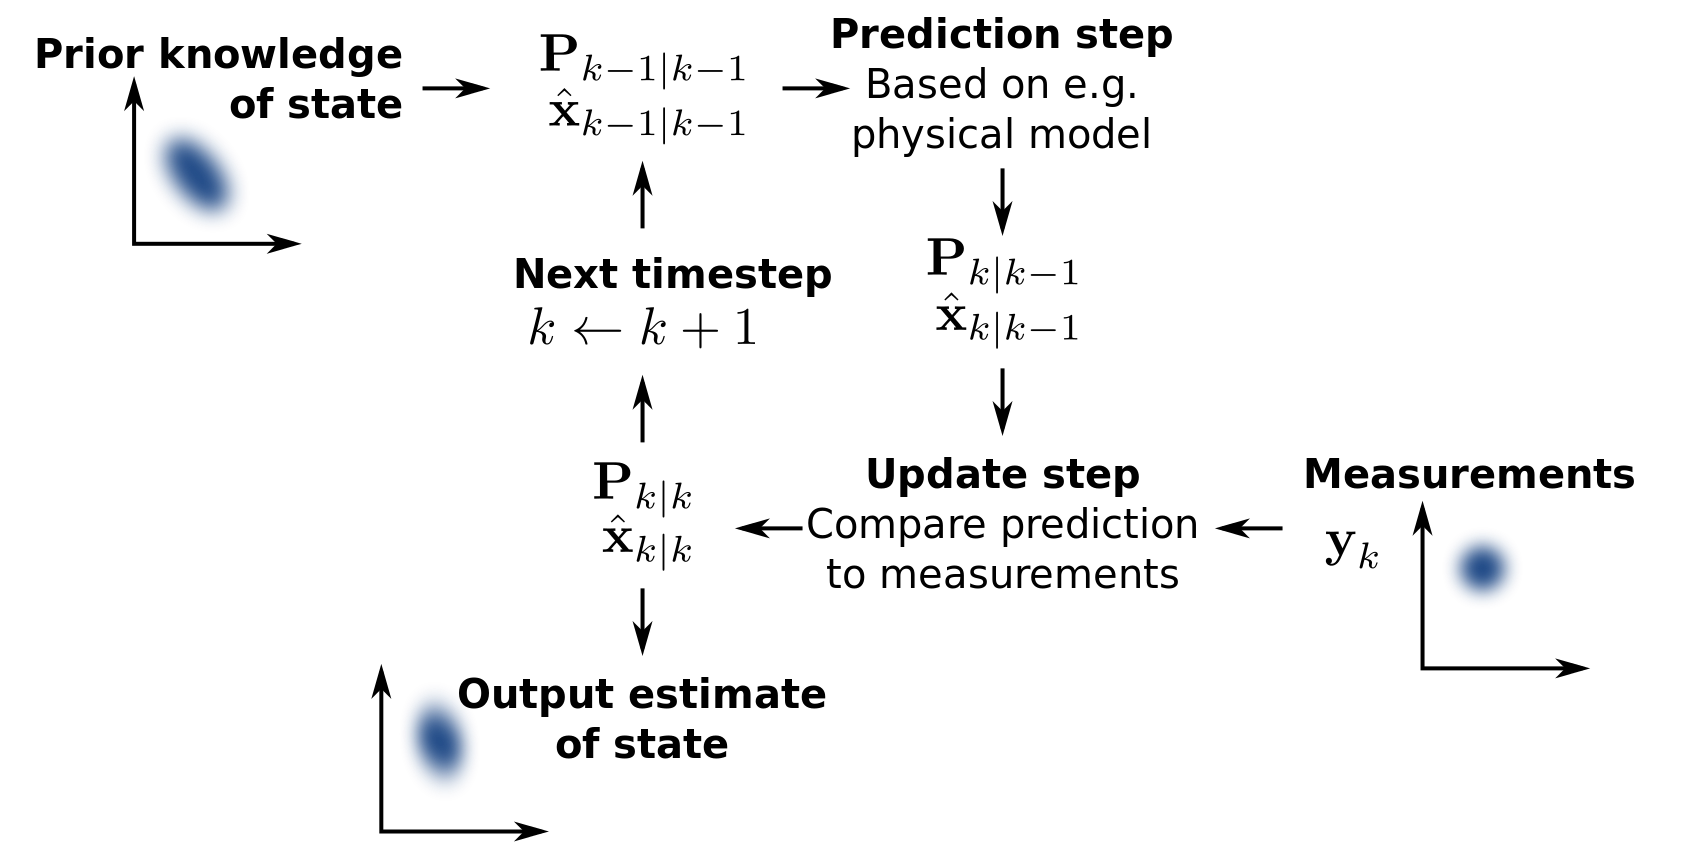
\includegraphics[scale = 0.2]{Images/kf/basic_sch.png}
    \caption[]{Kalman Filter two-step process.\textit{Font: Wikipedia}.}
    \label{fig:kf_sch}
\end{figure}%
The Kalman filter deals really well with uncertainty, it is able to reduce the sensor noise and process noise by the means of making the best guess in the estimate. The statistical algorithm has the property to be a recursive estimator, so it is only needed the previous state and the current measurement to predict the current state.
% Kalman filter prediction always, not only when we dont see the ball!!!!!

The state chosen in our system is considering the motion of the ball as shows eq.\ref{eq:kf_state}.

\begin{align}
    \mathrm{x_k} &= \begin{bmatrix}
           x, y, z, v_x, v_y, v_z, a_x, a_y, a_z
         \end{bmatrix}
    \label{eq:kf_state}
  \end{align}
The process and measurement covariances matrices should be defined In order to initialize the Kalman Filter. These matrices indicates the noise level in the measurement sensors (usually specified by the manufacturer) denoted as R and the noise in the process which is related to the noise in the state denoted as Q. For further information on the calculations for prediction and update steps see section \ref{sec:annex}.


